% Drzewiaste struktury danych
\section{Drzewiaste struktury danych}
\subsection{BST}
\entry
Drzewa wyszukiwań binarnych (drzewa BST – Binary Search Trees) - drzewa binarne, w których elementy
rozmieszczone są w porządku symetrycznym.

\entry
Właściwości BST:  

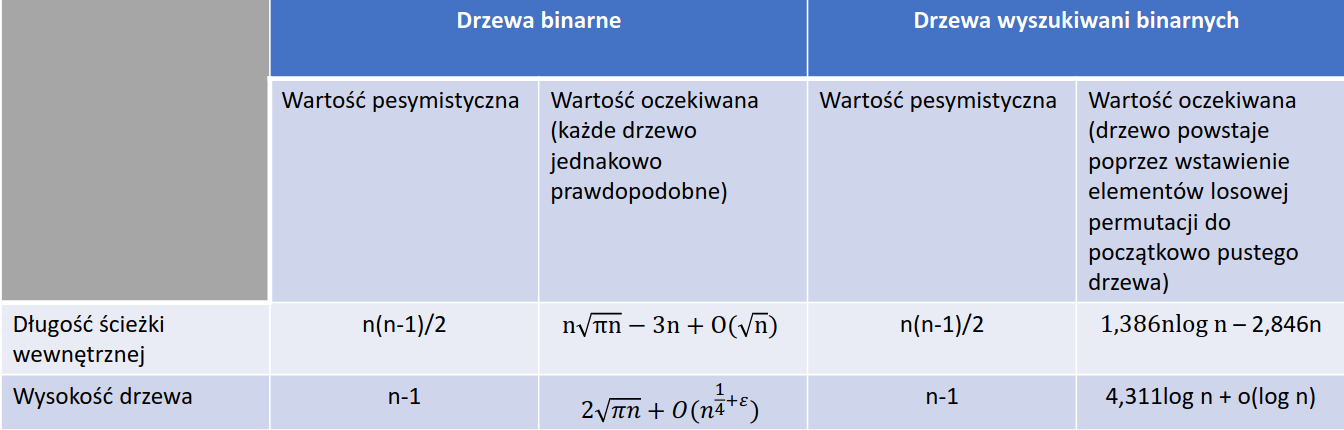
\includegraphics[scale=0.25]{drzewa1.png}

\subsection{AVL}
\entry
AVL-drzewo – drzewo wyszukiwań binarnych, w którym dla każdego węzła wysokości jego poddrzew
różnią się co najwyżej o 1

\entry
Złożoność operacji to $\log{n}$ gdzie n to wielkość drzewa.

\entry 
Atrybuty węzłów drzewa z wykładu:  

Key(v) – klucz  

Left(v), Right(v), Parent(v) – wskaźniki odpowiednio do lewego i prawego dziecka oraz rodzica  

Bf(v) – wskaźnik zrównoważenia (ang. balance factor) równy h(T(Left(v)) – h(T(right(v)) ∈ {-1, 0, 1}

\entry
Przyjmujemy, że węzeł zewnętrzny ma wysokość -1.

\entry
Rotacje zachowują porządek symetryczny w BST, numerację infiksową (inorder) węzłów drzewa binarnego!

\entry
Pojedyncza rotacja w prawo i lewo:  

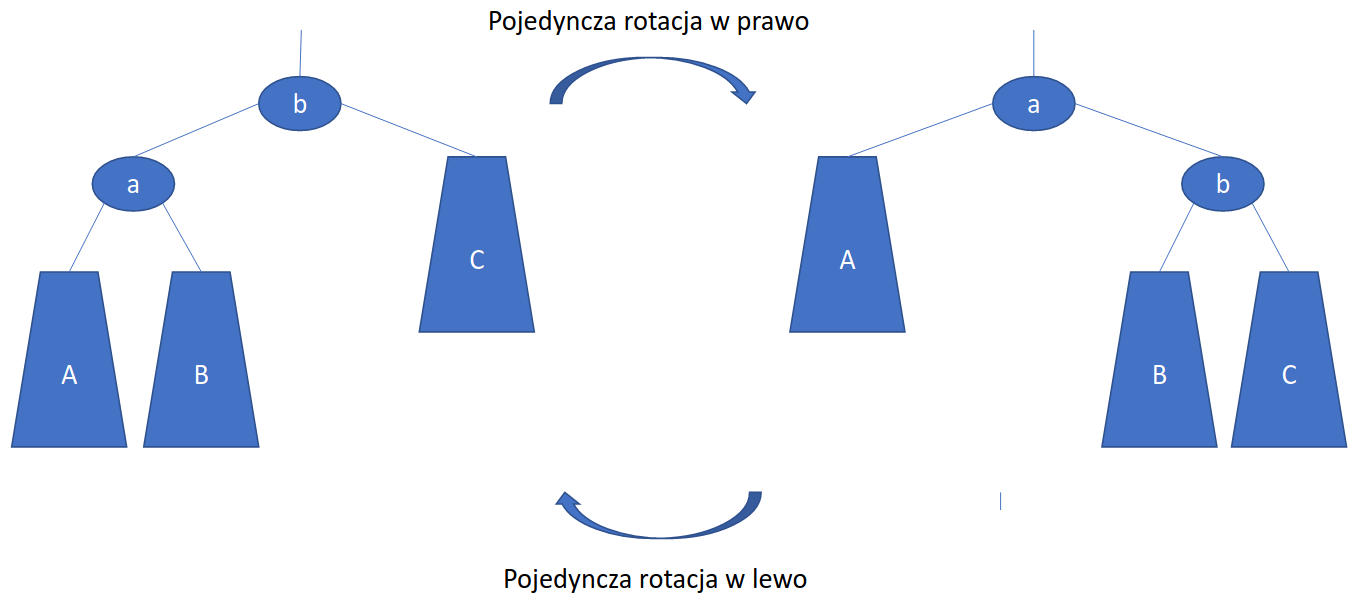
\includegraphics[scale=0.25]{pojedynczaRotacja.png}

\entry
Podwójna rotacja w prawo:  

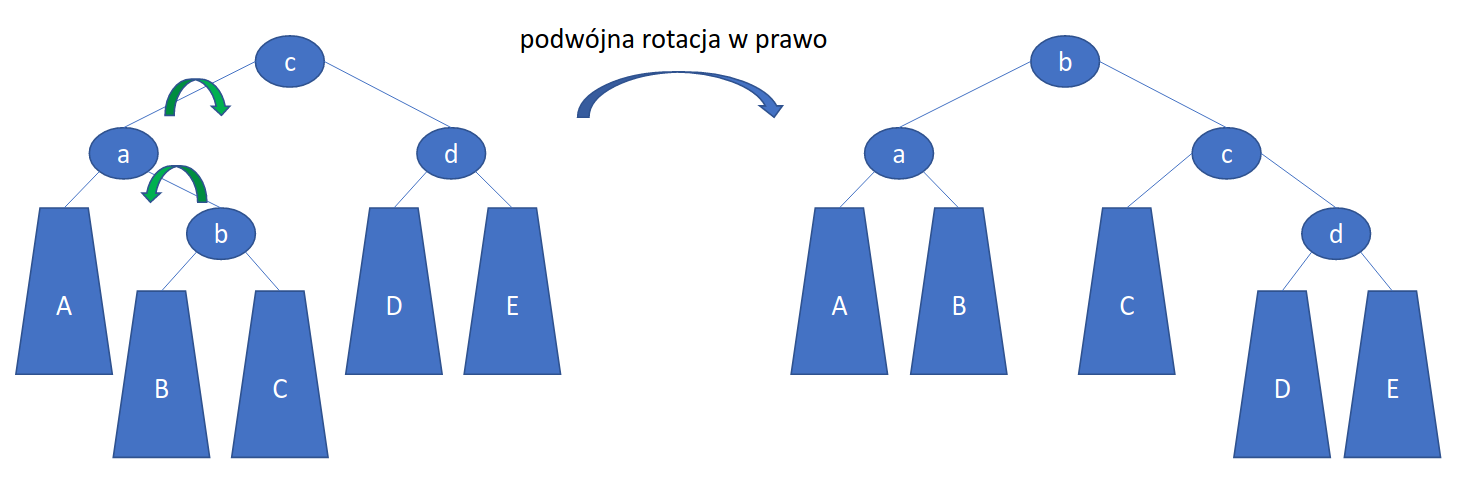
\includegraphics[scale=0.25]{podwojnaWPrawo.png}

\entry
Podwójna w lewo:

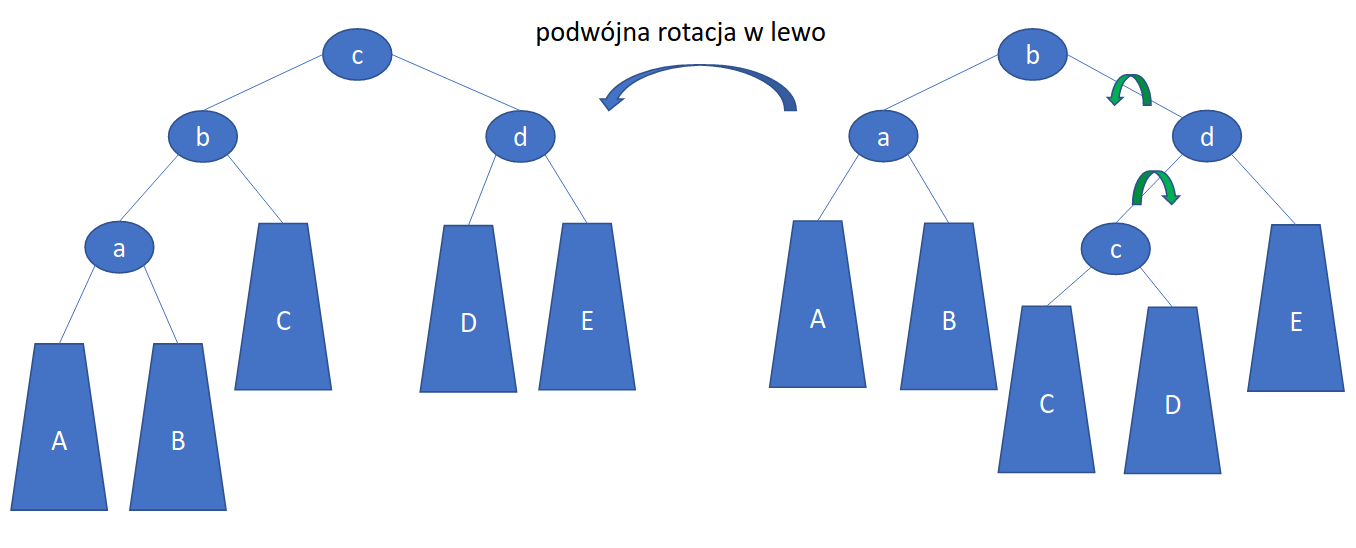
\includegraphics[scale=0.25]{podwojnaWLewo.png}

\entry
Schemat wstawiania elementu gdy urosło lewe poddrzewo(symetrycznie dla prawego):

Bf v = -1 $\Rightarrow$ Bf v = 0; STOP

Bf v = 0 $\Rightarrow$ Bf v = 1; $\Uparrow$ (poprawiaj w górę)

Bf v = 1 $\Rightarrow$ rotacja

\entry
Schemat usuwania elementu gdy zmalało lewe poddrzewo(symetrycznie dla prawego):

Bf v = −1 $\Rightarrow$ rotacja

Bf v = 0 $\Rightarrow$ Bf v = −1; STOP

Bf v = 1 $\Rightarrow$ Bf v = 0; $\Uparrow$ (poprawiaj w górę)

\entry
Wzbogacenia AVL przedstawione na wykładzie:

OnLeft(v) – liczba węzłów w lewym poddrzewie v

Max(v) – maksimum z elementów w poddrzewie o korzeniu v

\entry
Rotajce w drzewie zachowują kolejność infiksową(inorder)

\subsection{Splay}
\entry
Operacje na drzewach splay są w czasie zamortyzowanym logarytmicznym

\entry
Podczas każdej operacji na drzewie splay wierzchołek, na którym wykonujemy operację, staje się korzeniem.

\entry
Local Splay:

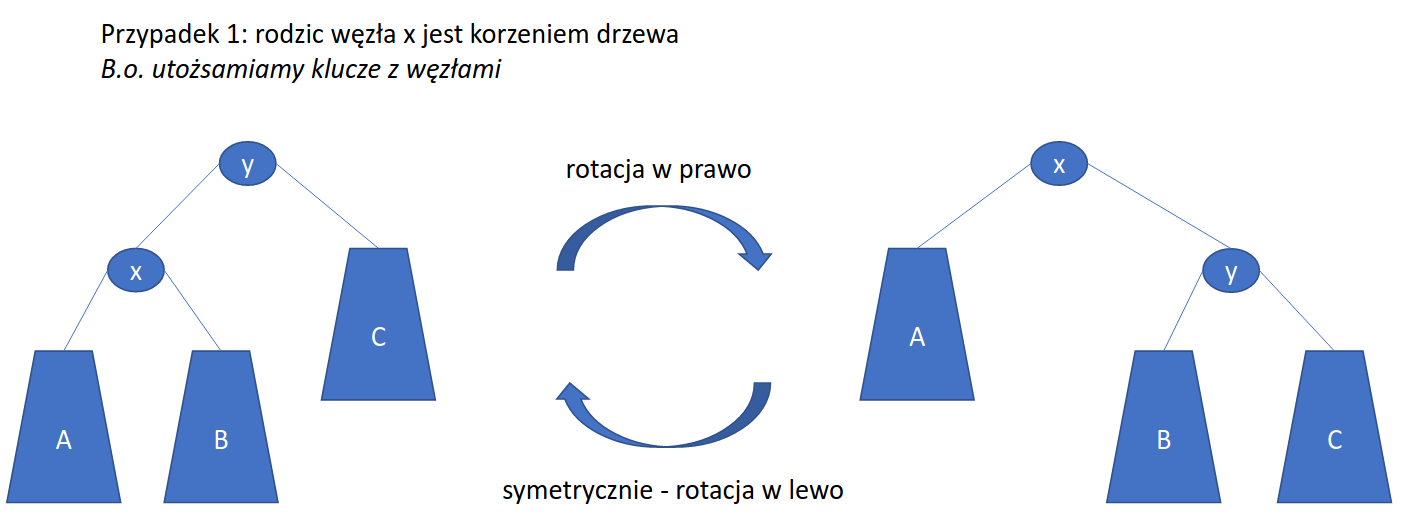
\includegraphics[scale=0.25]{splay1.png}

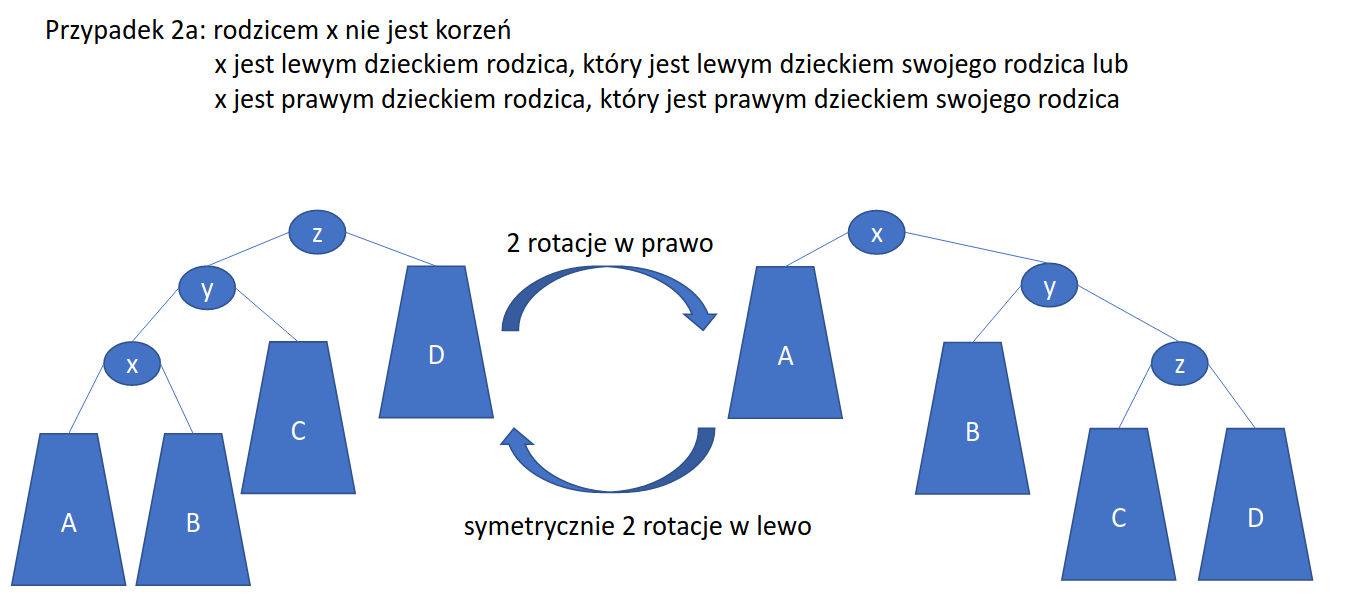
\includegraphics[scale=0.25]{splay2.png}

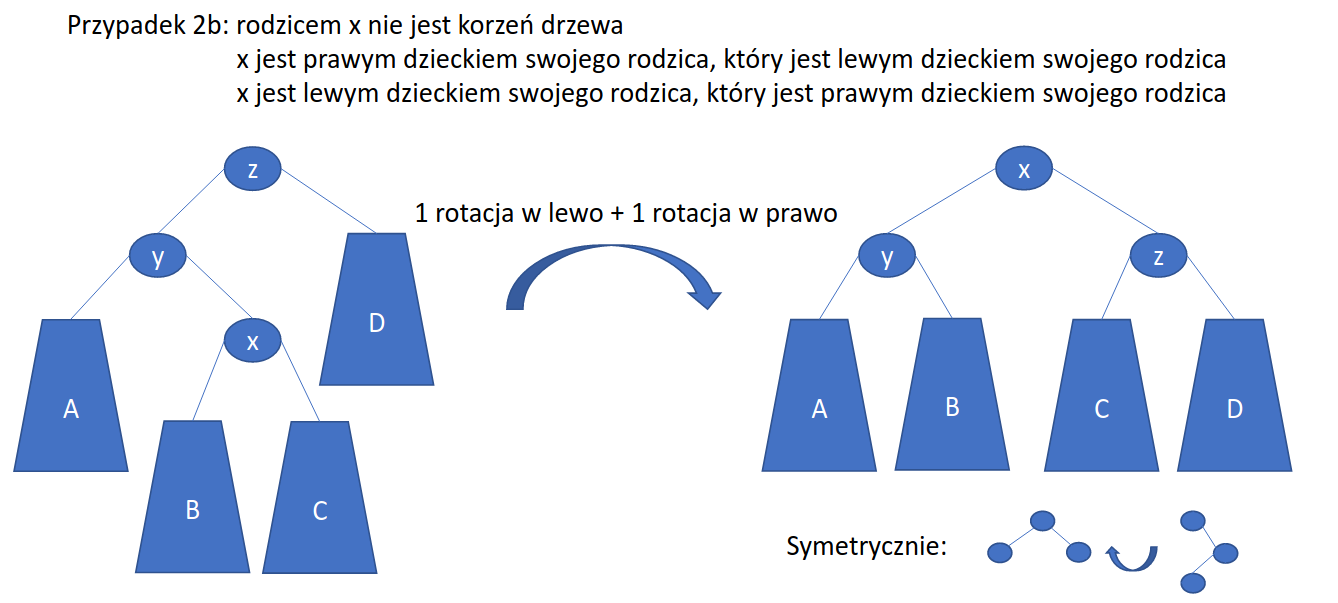
\includegraphics[scale=0.25]{splay3.png}

\entry 
Istnieje operacja split która dzieli drzewo na dwa poddrzewa według wieżchołka v. (lewe drzewo ma klucze mniejsze a prawe wieksze niż klucz v)

\subsection{Drzewa B}
\entry
Niech t będzie liczbą całkowitą większą od 1.

B-drzewem (minimalnego) stopnia t nazywamy drzewo z korzeniem spełniające poniższe warunki:

• Każdy węzeł x ma następujące atrybuty:

a) m – liczba kluczy aktualnie pamiętanych w x

b) m kluczy Key1, Key2, ..., Keym uporządkowanych rosnąco (załóżmy ponadto, że mamy
wirtualnych strażników Key0 = -∞ oraz Keym+1 = +∞)

c) Leaf – atrybut logiczny przyjmujący wartość TRUE wiw, gdy x jest liściem

• Każdy węzeł wewnętrzny x zawiera m+1 wskaźników P1, P2, ..., Pm+1 do swoich dzieci w drzewie.
Dla liści wartością tych wskaźników jest NULL.

• Każdy klucz K w poddrzewie wskazującym przez Pi spełnia warunek Keyi-1 < K < Keyi.

• Wszystkie liście leżą na tej samej głębokości równej wysokości drzewa h.

• Każdy węzeł różny od korzenia całego drzewa musi zawierać co najmniej t-1 i co najwyżej 2t-1
kluczy (odpowiednio, co najmniej t i co najwyżej 2t wskaźników do dzieci, o wartościach
równych NULL jeśli jest to liść).

• W niepustym drzewie korzeń musi zawierać, co najmniej 1 i co najwyżej 2t-1 kluczy (odpowiednio
co najmniej 2 i co najwyżej 2t wskaźników do dzieci - o wartościach NULL, jeśli jest to
jednocześnie liść).

\entry 
Złożoności

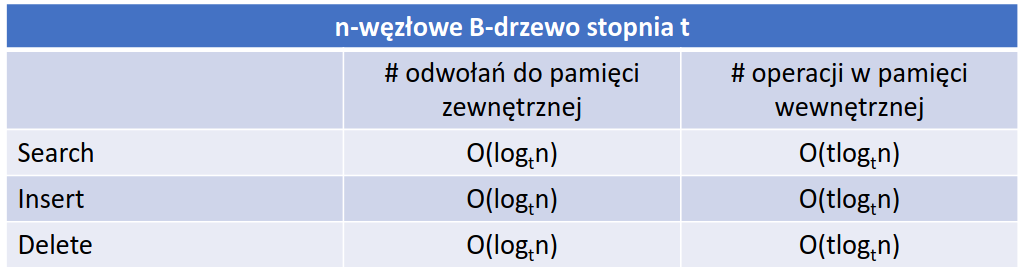
\includegraphics[scale=0.35]{boperacje.png}

\entry 
B-drzewo o (minimalnym) stopniu t = 2 nazywamy 2-3-4-drzewem (każdy węzeł, nie liść, ma 2 lub 3 lub 4 dzieci)

\entry
Korzeń poddrzewa do którego wchodzimy, różny od korzenia, nigdy nie jest minimalny!

\entry
Korzeń poddrzewa do którego wchodzimy nigdy nie jest maksymalny!

\entry
Wysokość drzewa: $h \leq \log_t(\frac{n+1}{2})$

\entry
Przykład drzewa

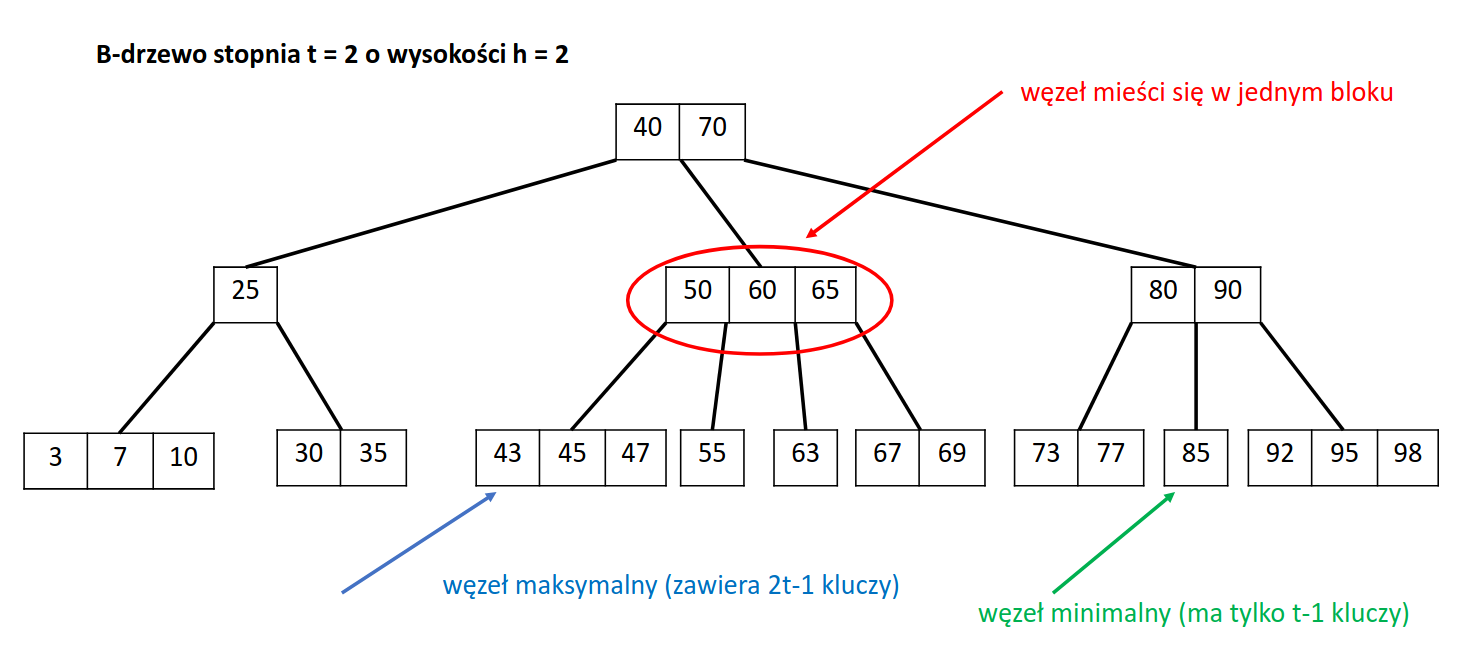
\includegraphics[scale=0.25]{bprzyklad.png}

\subsection{Drzewa Czerwono Czarne}

\entry
Drzewo czerwono-czarne – drzewo BST, w którym każdy węzeł jest pokolorowany
na czerwono lub czarno zgodnie z następującymi regułami:

1. korzeń drzewa jest czarny

2. każdy czerwony węzeł ma czarnego rodzica

3. każdy węzeł zewnętrzny (NULL) jest czarny

4. każda ścieżka (elementarna) z ustalonego węzła do węzła zewnętrznego w jego
poddrzewie zawiera tyle samo węzłów czarnych

\entry
Wysokość drzewa wynosi $h \leq 2 \log_2(\frac{n+1}{2})$

\entry
Slajdy

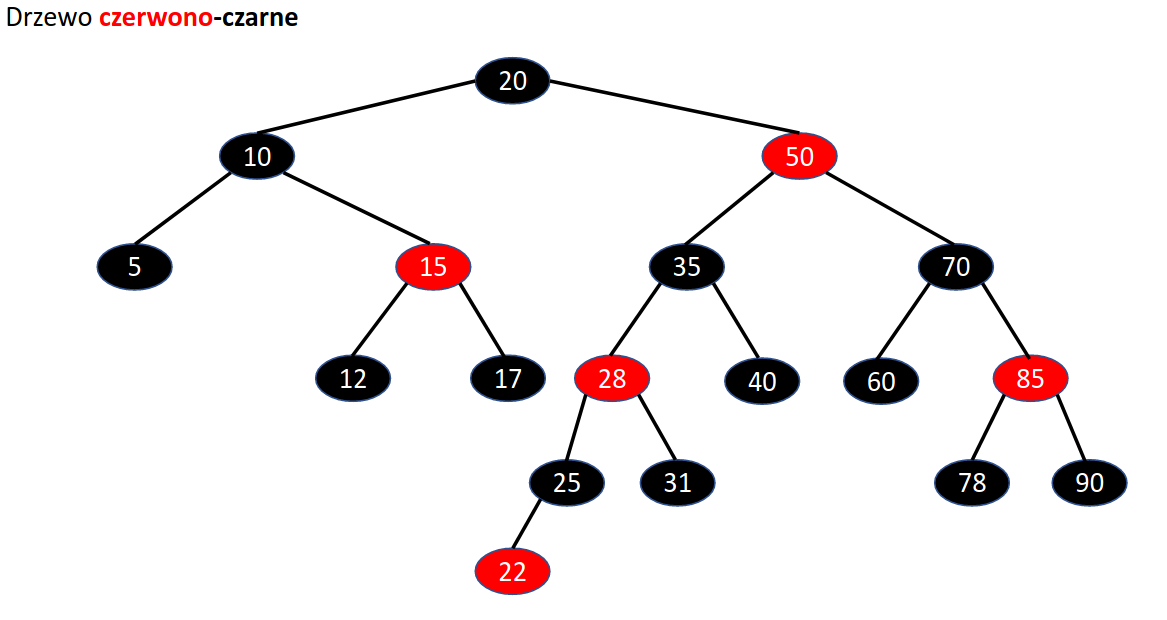
\includegraphics[scale=0.25]{cc1.png}

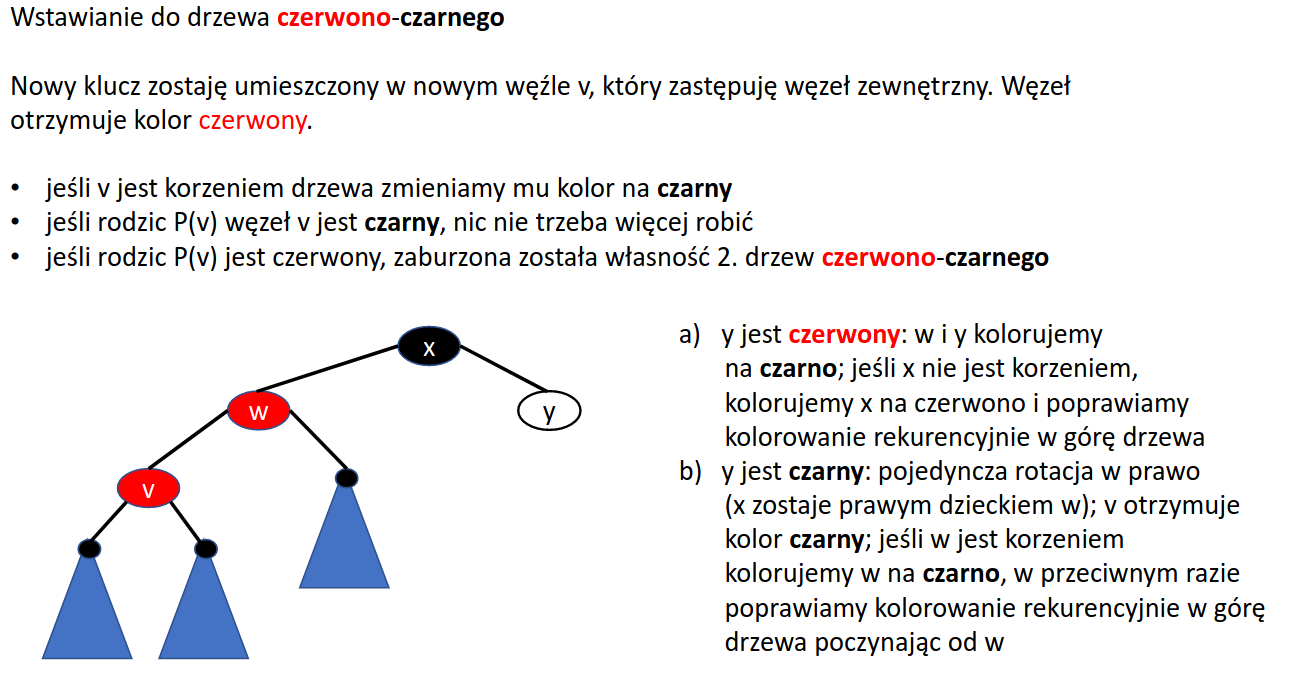
\includegraphics[scale=0.25]{cc2.png}

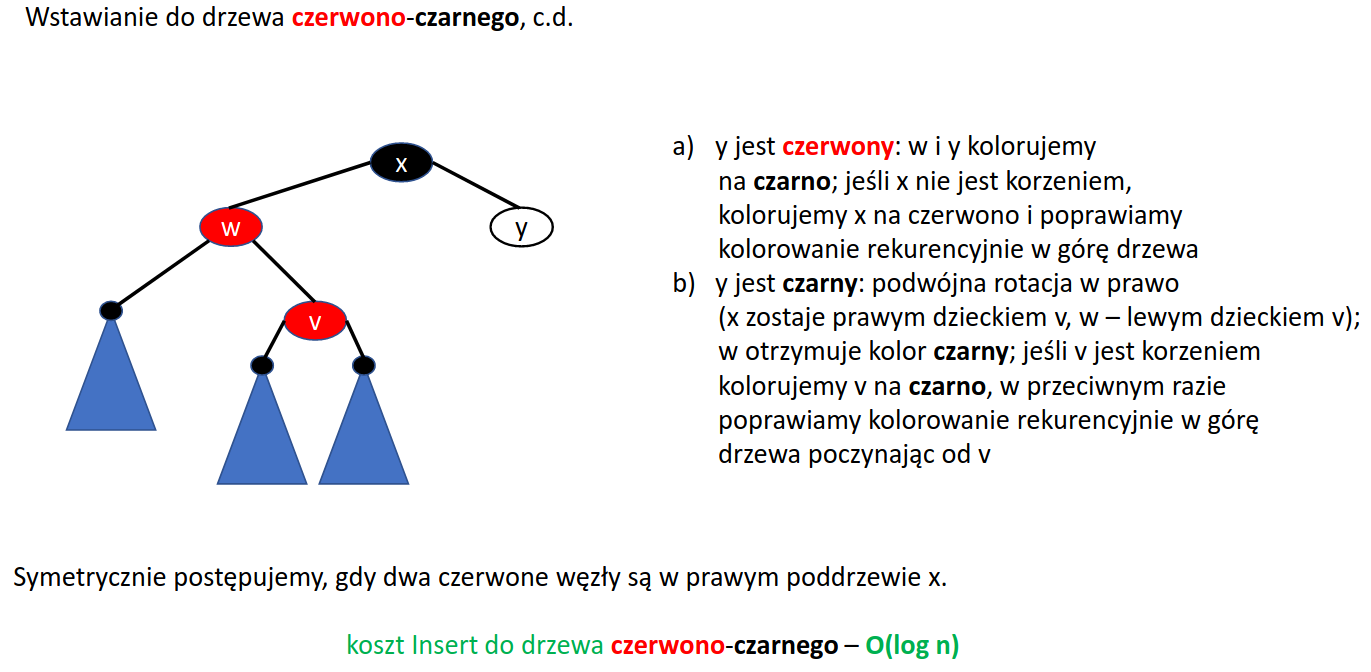
\includegraphics[scale=0.25]{cc3.png}

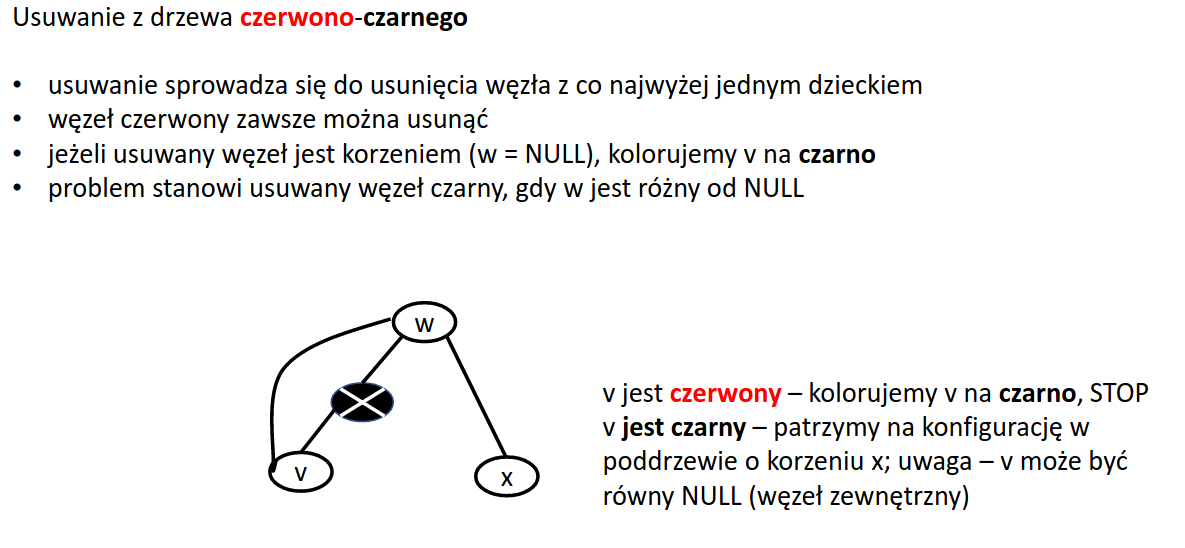
\includegraphics[scale=0.25]{cc4.png}

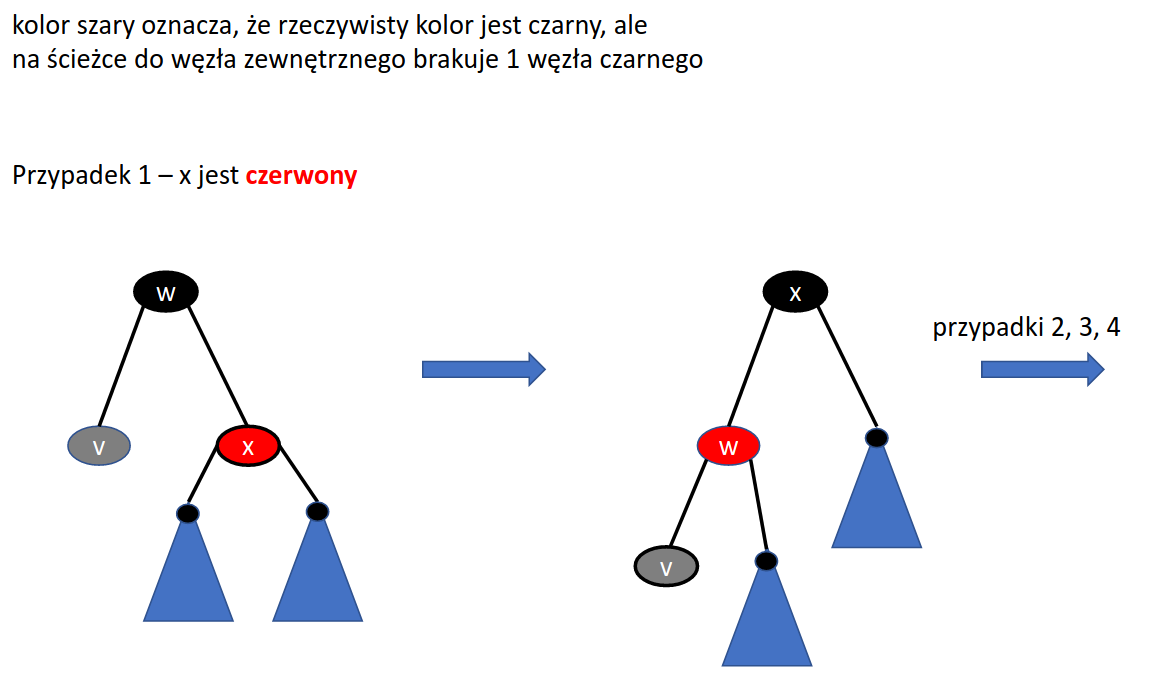
\includegraphics[scale=0.25]{cc5.png}

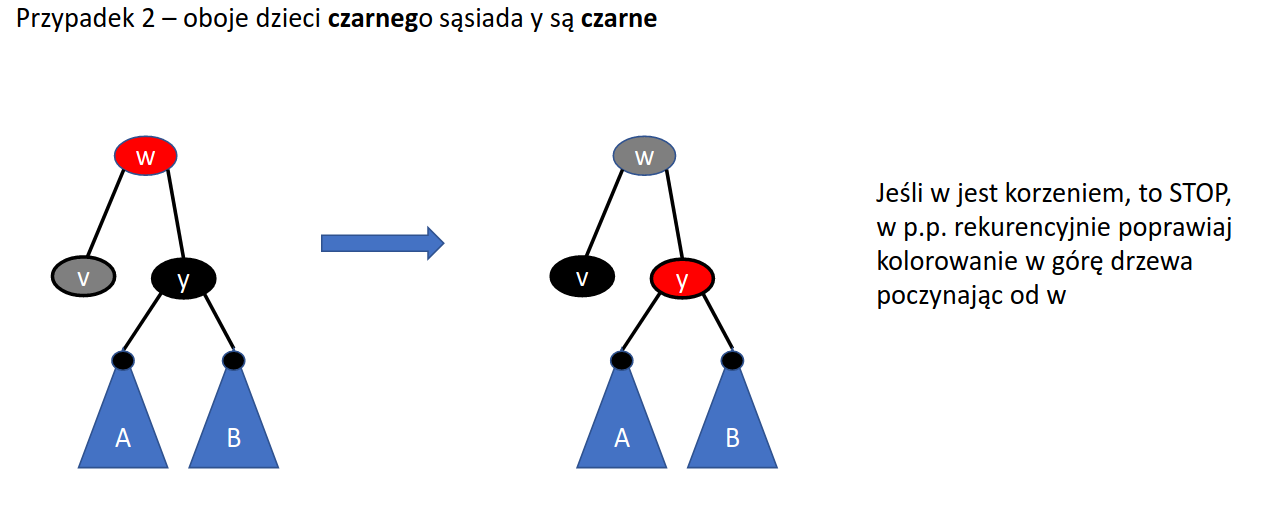
\includegraphics[scale=0.25]{cc6.png}

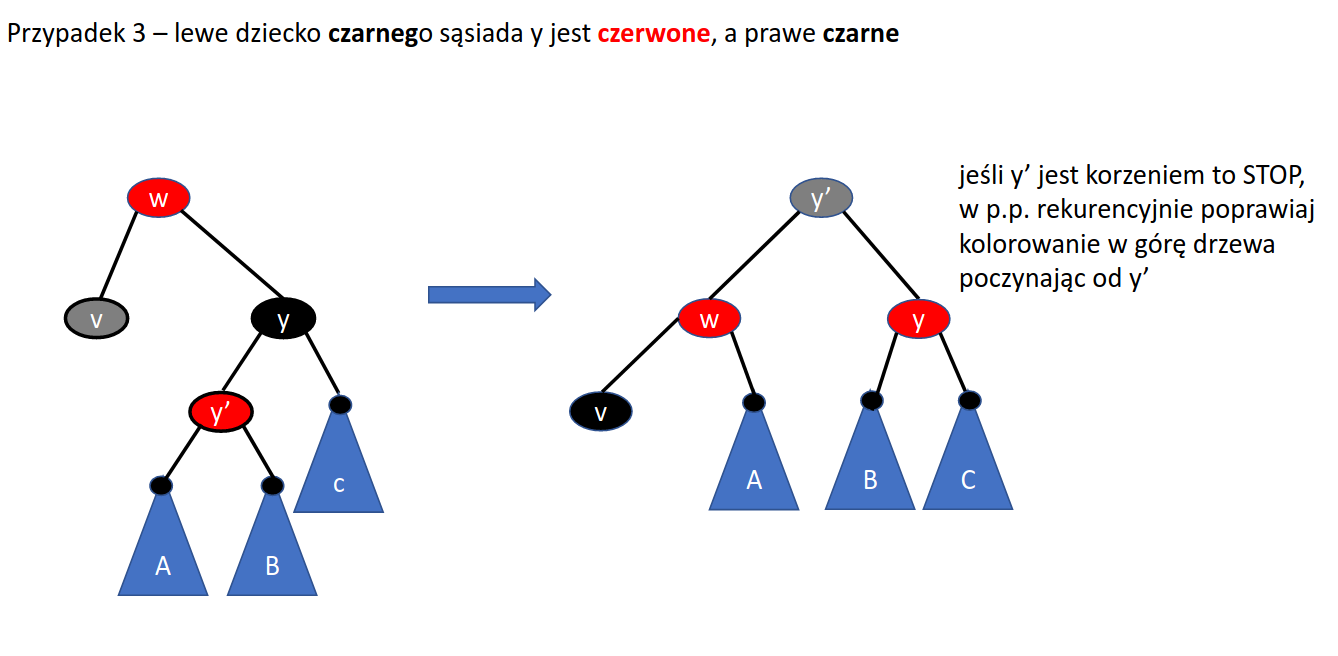
\includegraphics[scale=0.25]{cc7.png}

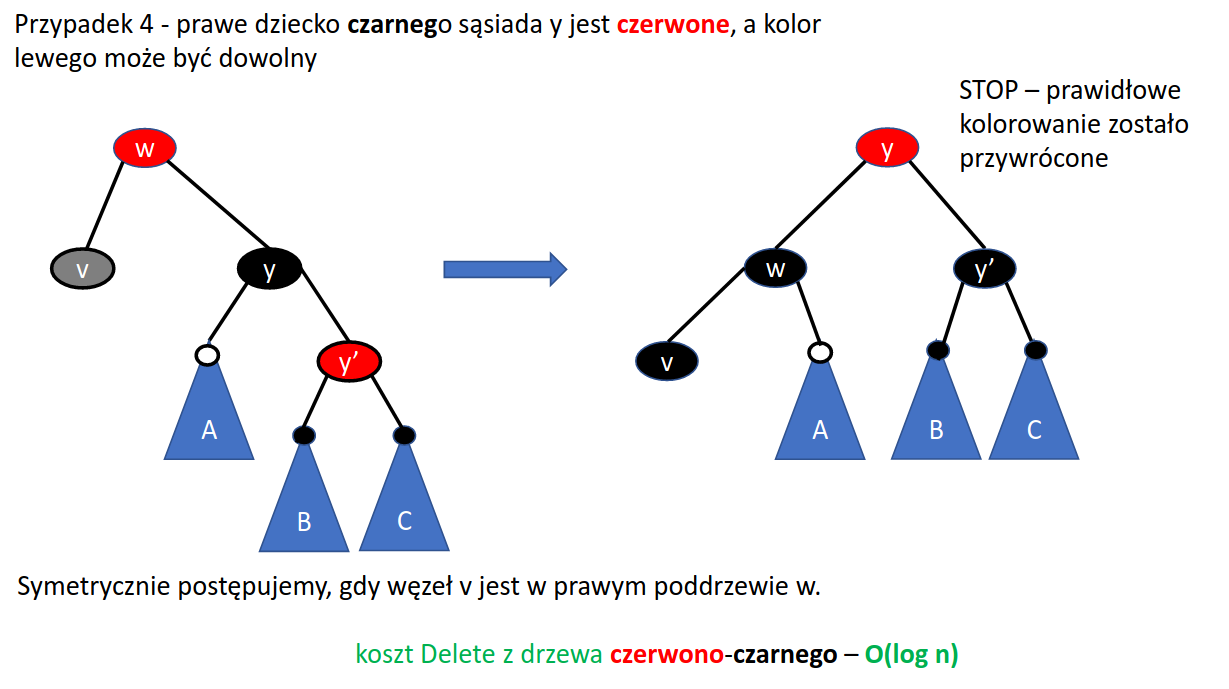
\includegraphics[scale=0.25]{cc8.png}

